\documentclass{article}
\usepackage[utf8]{inputenc}
\usepackage{amsmath}
\usepackage{geometry}
\usepackage[utf8]{inputenc}
\usepackage{graphicx}
\usepackage{caption}
\geometry{a4paper, margin=1in}
\usepackage{hyperref}
\usepackage{subcaption}

\title{Data Management Project}
\author{Oleksandr Kasat}
\date{}

\begin{document}

\maketitle

\section*{Introduction}

The project was primarily focused on analyzing music trends and how they are influenced by various factors: cultural, social, and possibly even industrial (e.g., do music services differ in terms of their user segments?). I found some answers, though nothing truly surprising. I attribute this to several reasons: globalization and the gradual merging of different cultures, as well as the limited transparency of data provided by music services, which prevents thorough analysis of certain patterns.

I believe the music industry today is quite open and does not necessarily need additional representation. However, I worked with a well-known music statistics resource: \textbf{kworb.net}, which collects a significant amount of data from the most popular music platforms, starting from 2011. Initially, I also considered incorporating data from another popular source — \url{http://www.mediatraffic.de/}, but I eventually realized that it would scale the project to an unmanageable size. The files were already quite large (e.g., 5 years of data = 500MB).

To parse the data, I decided to use Selenium instead of BeautifulSoup. The website required dynamic crawling due to the presence of pop-ups, ads, and cookie banners. Therefore, I opted for a tool capable of handling such elements. The parser navigates through all sections of the site and processes them. Some parts required manual interaction (like clicking through pages), while others were easier to load — each section had its own structure. I tried to design general-purpose functions based on recurring patterns and reused them where possible throughout the parsing process.

After parsing the site, I obtained about 35 tables. Through data cleaning and concatenation, I created a new database consisting of 11 cleaned tables.

\begin{itemize}
    \item \textbf{Spotify:} Two tables (daily and weekly aggregations) containing basic attributes describing Spotify chart data.
    \begin{itemize}
        \item \textbf{Artist and Title}
        \item \textbf{Wks} – Number of weeks in the chart
        \item \textbf{T10} – Days in the Top 10 before the current snapshot (some entries may have missing values)
        \item \textbf{Peak (x?)} – Highest chart position achieved (x = number of times it was reached)
        \item \textbf{PeakStreams} – Highest number of daily streams received
        \item \textbf{Total} – Total number of streams at the snapshot moment
    \end{itemize}
    Three additional tables (Artists, Listeners, Top List):
    \begin{itemize}
        \item \textbf{Artists} – Most streamed artists of all time with availability to check which kind ot traffic it is (solo songs or featuring with someone)
        \item \textbf{Listeners} – Shows recent trends (daily +/- changes) and peak listener values
        \item \textbf{Top Lists} – Top-streamed songs across different eras. Honestly, I didn`t use it much.
    \end{itemize}
    
    \item \textbf{iTunes Archive / Cumulative:}  
    The archive table provides hourly sales data for each track. At first glance, the headers may seem confusing, but they indicate the relative sales performance of a song X hours before a specific snapshot (e.g., June 19, 2017). For example, a value of 0.2658 means the song had only 26.58\% of the sales of the current number one track. The cumulative table aggregates the total sales to produce a ranking over a defined period.
    
    \item \textbf{Archive Albums / Songs:}  
    Since iTunes primarily reports sales figures, assessing popularity based on recent streaming is difficult. Kworb.net attempts to address this by calculating rankings using regional data. Over 100 countries are included and grouped based on consumption characteristics. These values are combined into a final 'Points' score. The tables are separated by platform (iTunes / Apple Music) and by region (Europe / World), and they are archived for temporal analysis.

    \item \textbf{Radio Charts Archive:}  
    Contains data related to radio airplay, including how many days a track has been played on certain stations (\textit{Days}), its total audience and change from the previous day (\textit{Aud}, \textit{Aud+}), and how many formats/stations broadcasted the track. Although the author also included some data from music services, I didn’t find it particularly useful. The tables are based on data from All Access, processed and uploaded by the site owner.

    \item \textbf{YouTube Clips:}  
    This section includes the most popular music videos by year. Each table contains 500 samples, covering 14 years, plus older viral videos from before the 2010s.
\end{itemize}

\bigskip

I followed a fairly straightforward pipeline: parse the data → preprocess it → generate insightful graphs → develop a web application to present the results. I believe a web app is the most transparent and interactive way to represent such findings, especially for data specialists.

\smallskip

Although the data were already partially processed by the source, I needed to engineer additional features and clean up some inconsistencies. It’s hard to generalize the dataset characteristics because I worked with the 5-years version of the data (~500MB; for example, the \textit{archive\_albums} table had over one million entries). I used SQLite3 to build the database, as it is suitable for small to medium-sized datasets and integrates well with Flask. For visualization, I chose Plotly because it offers intuitive web integration through Plotly.js. Throughout the analysis, I aimed to identify patterns in the dataset, and the resulting graphs are primarily based on these observations.\\

\clearpage

\section*{Overall Analysis}

\begin{figure}[htbp]
    \centering
    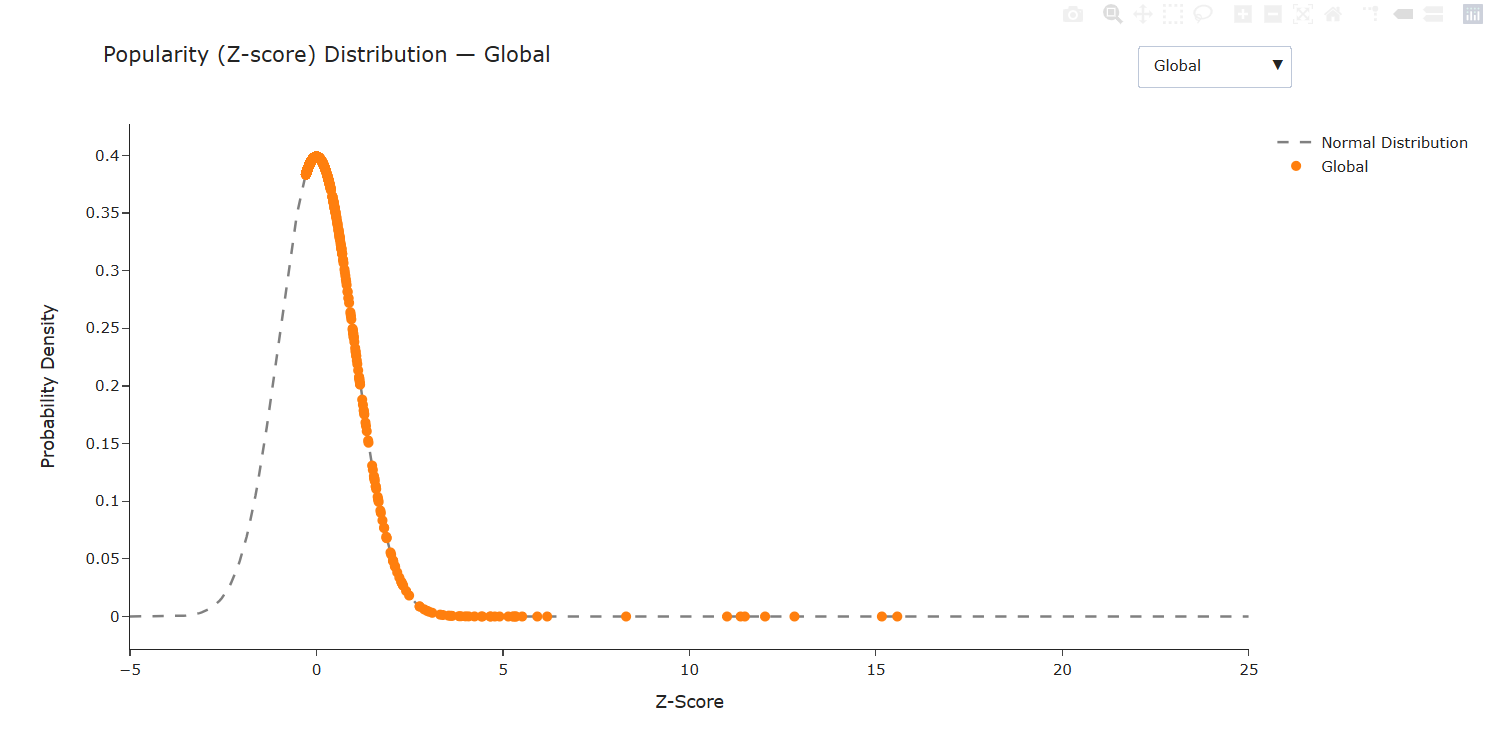
\includegraphics[width=0.8\textwidth]{data/report_figures/graph1_spotify.png}
    \caption{\textbf{Popularity Distribution} \\
    This graph illustrates the Z-distribution of an artist's popularity within a specific region, calculated as a ratio of the artist's total streams to the overall streams across all artists in that region. Logarithmic transformation is applied for a steadier distribution, revealing that some artists 	significantly deviate from the norm, which is typical in the music industry. As you can see, even this transformation didn`t help a lot. So the distribution is obviously right-skewed, because there are 5-10 artists which are many times more popular than the rest. It could be affected the grobalization processes and more advanced
recommendation systems which feed us only the most popular ones, and every day it becomes more and more difficult for the average person to find a niche artist.}
    \label{fig:spotify1}
\end{figure}

\begin{figure}[htbp]
    \centering

    \begin{subfigure}[b]{0.8\textwidth}
        \centering
        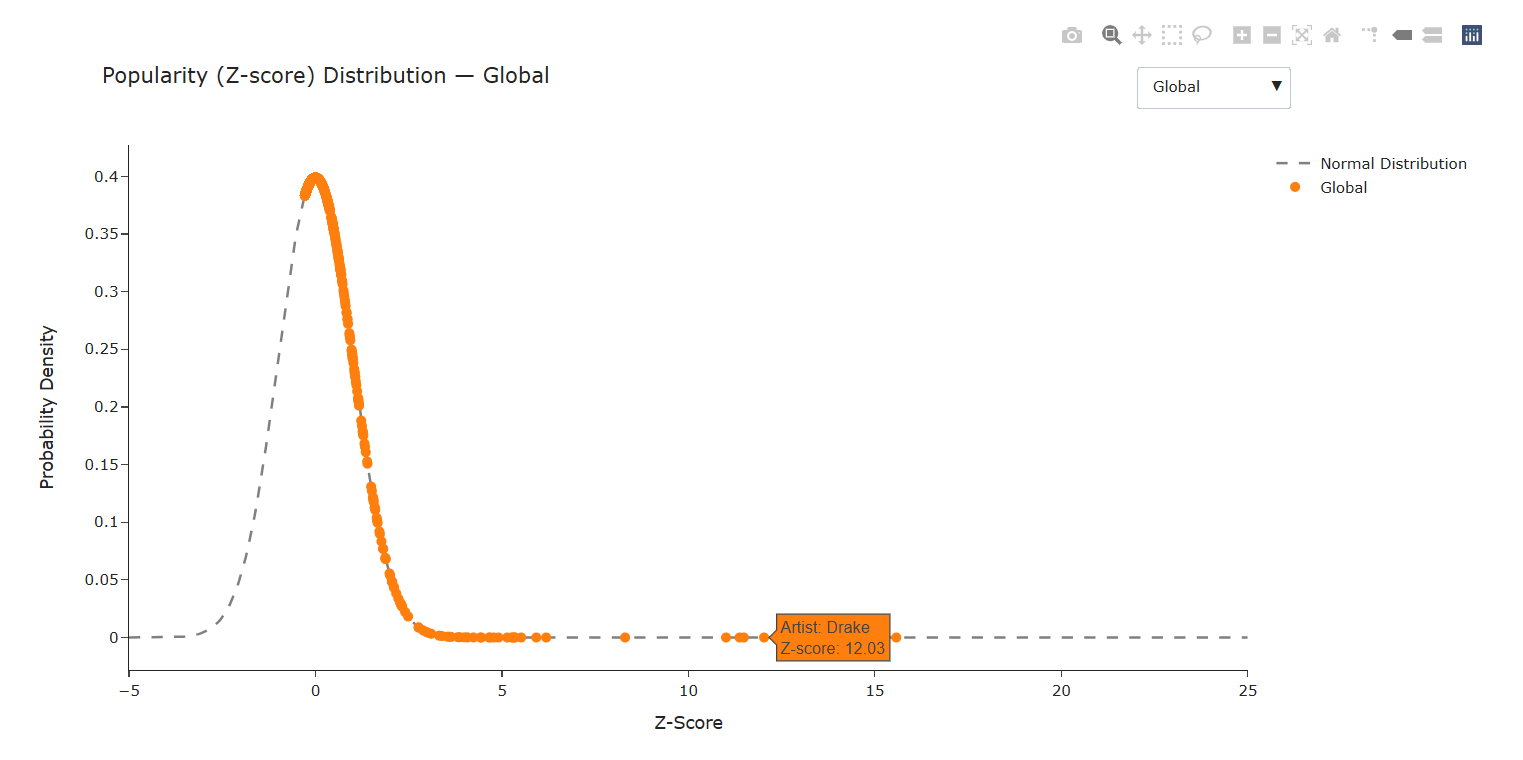
\includegraphics[width=\textwidth]{data/report_figures/graph2_spotify.png}
        \caption{Z-distribution of an artist's popularity (Global)}
        \label{fig:spotify2}
    \end{subfigure}
    \vskip\baselineskip
    \begin{subfigure}[b]{0.8\textwidth}
        \centering
        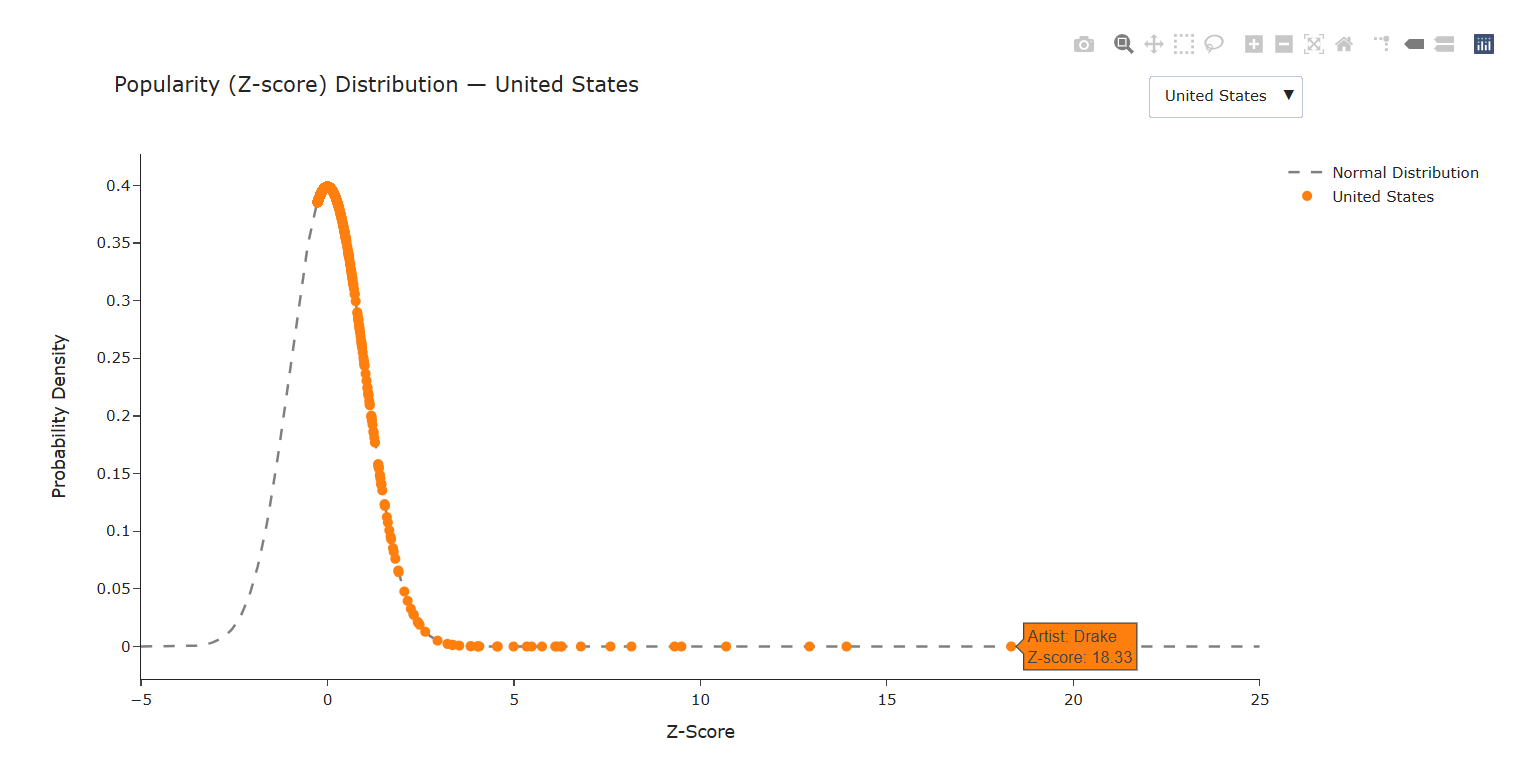
\includegraphics[width=\textwidth]{data/report_figures/graph3_spotify.png}
        \caption{Z-distribution of an artist's popularity (United States)}
        \label{fig:spotify3}
    \end{subfigure}

    \caption{\textbf{No differences in distribution between the US and the world} \\ 
    The most popular artists (Drake, Taylor Swift and Post Malone) and the right part of the graph in general create clusters that are located very close to each other. This suggests a great deal of influence from American culture on the rest of the world, but for a more thorough analysis we would also need to look at the left side of the graph, which is not possible to show in the report.}
    \label{fig:spotify_combined1}
\end{figure}

\clearpage

\begin{figure}[htbp]
    \centering
    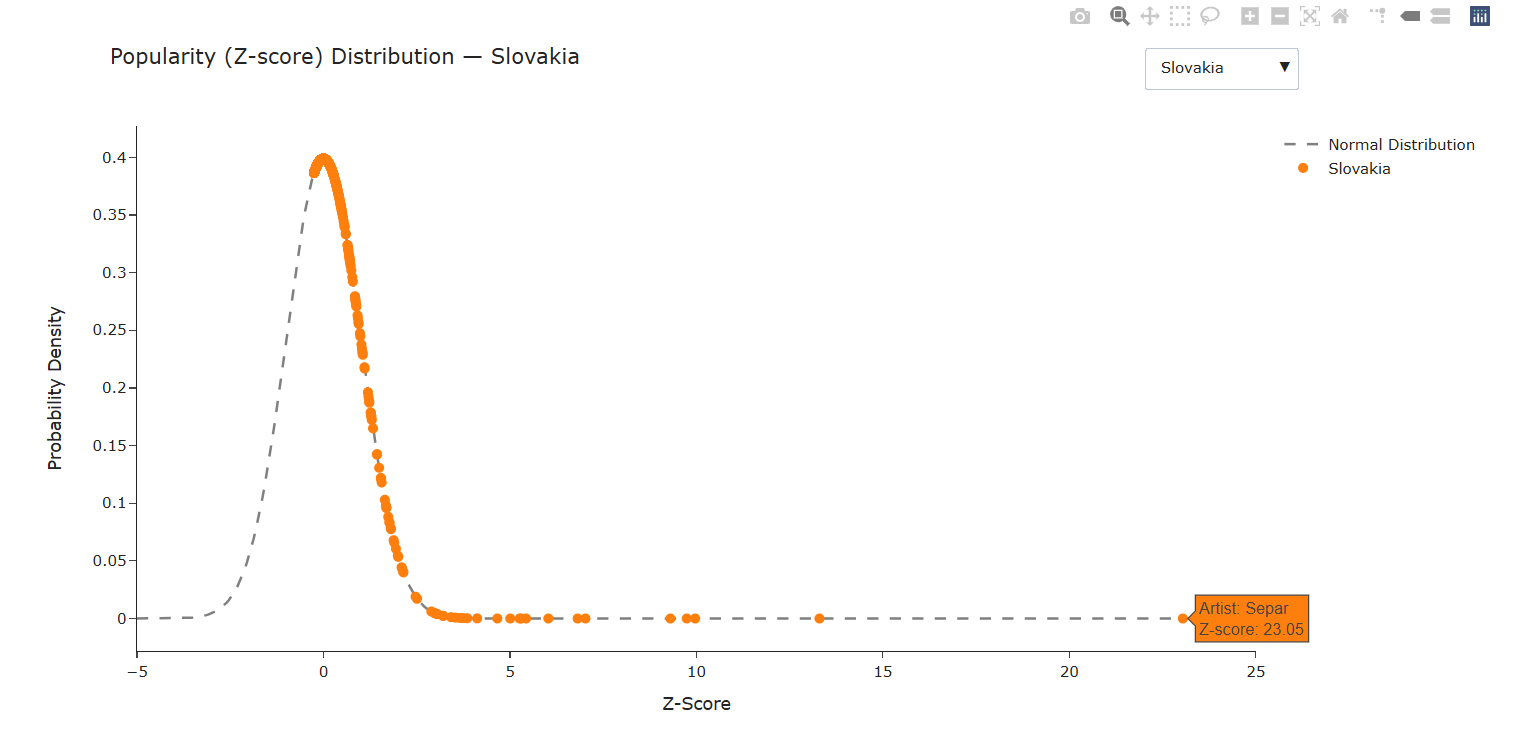
\includegraphics[width=0.8\textwidth]{data/report_figures/graph4_spotify.png}
    \caption{\textbf{Popularity of local artists within specific countries} \\
    The graph shows that specifically within the country, local musicians are many times more popular than world-famous ones, despite the general globalization. Moreover, these connections are many times stronger. Specifically in Slovakia, Czech performers also gain popularity. For example, in addition to the performer indicated on the graph, there are about a dozen more local musicians behind him, who are ahead of the world-famous artist (The Weeknd).}
    \label{fig:itunes1}
\end{figure}

\begin{figure}[htbp]
    \centering

    \begin{subfigure}[b]{0.8\textwidth}
        \centering
        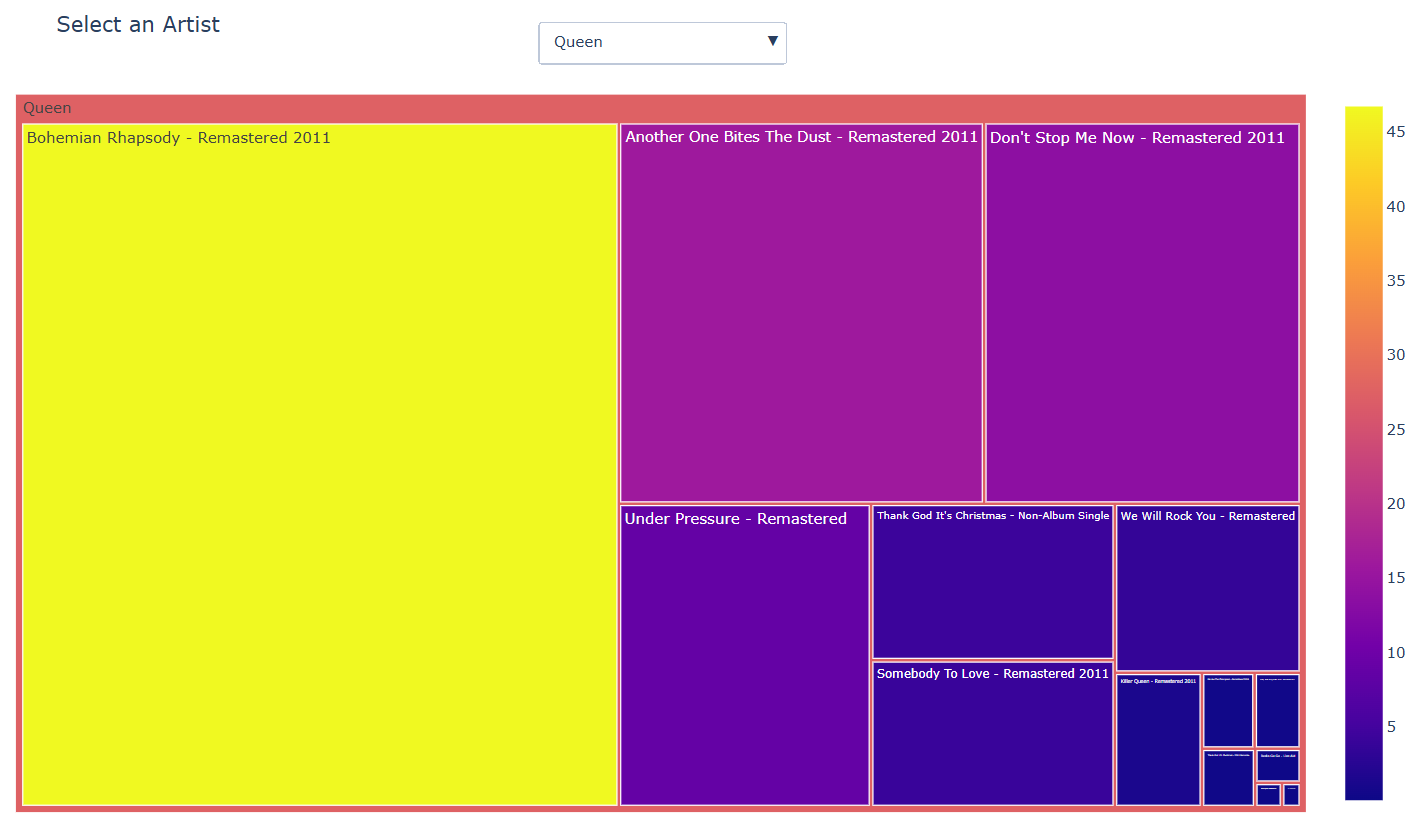
\includegraphics[width=\textwidth]{data/report_figures/graph5_spotify.png}
        \caption{Queen: the most popular songs}
        \label{fig:spotify5}
    \end{subfigure}
    \vskip\baselineskip
    \begin{subfigure}[b]{0.8\textwidth}
        \centering
        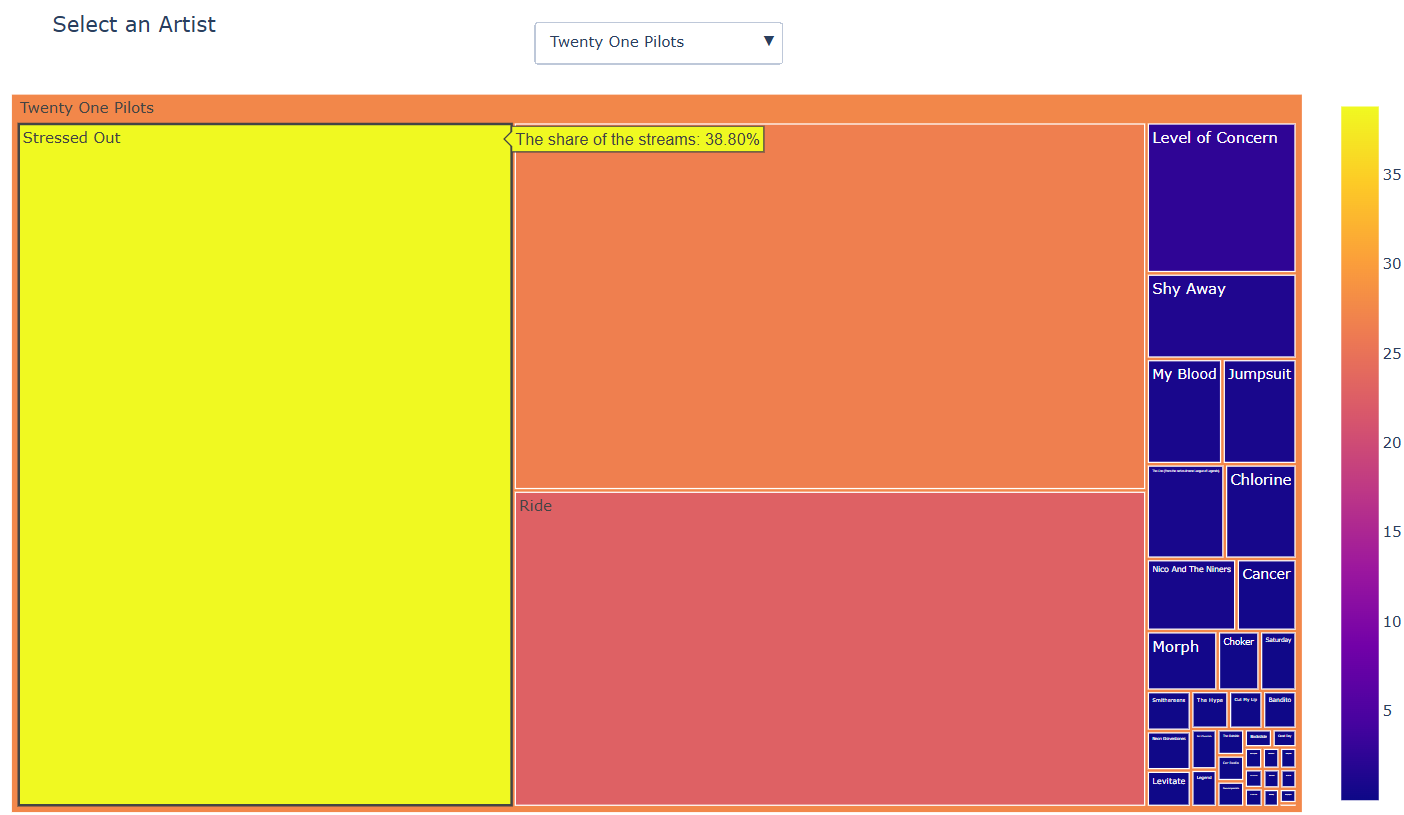
\includegraphics[width=\textwidth]{data/report_figures/graph6_spotify.png}
        \caption{Twenty One pilots: the most popular songs}
        \label{fig:spotify6}
    \end{subfigure}

    \caption{\textbf{Even the most popular artists and bands have tracks that are many times more popular than all other tracks by the same artist.} \\ 
    The chart itself is mostly interactive, it's hard to find any relations. But if you look at the charts for Queen and 21 Pilots separately, you'll notice that the majority of all listening is done by a small group of tracks. The second group has 3 tracks that take up 90\% of listening. But this only shows that it's not always possible to say that a group is a one-hit wonder.}
    \label{fig:spotify_combined2}
\end{figure}

\clearpage

\begin{figure}[htbp]
    \centering

    \begin{subfigure}[b]{0.8\textwidth}
        \centering
        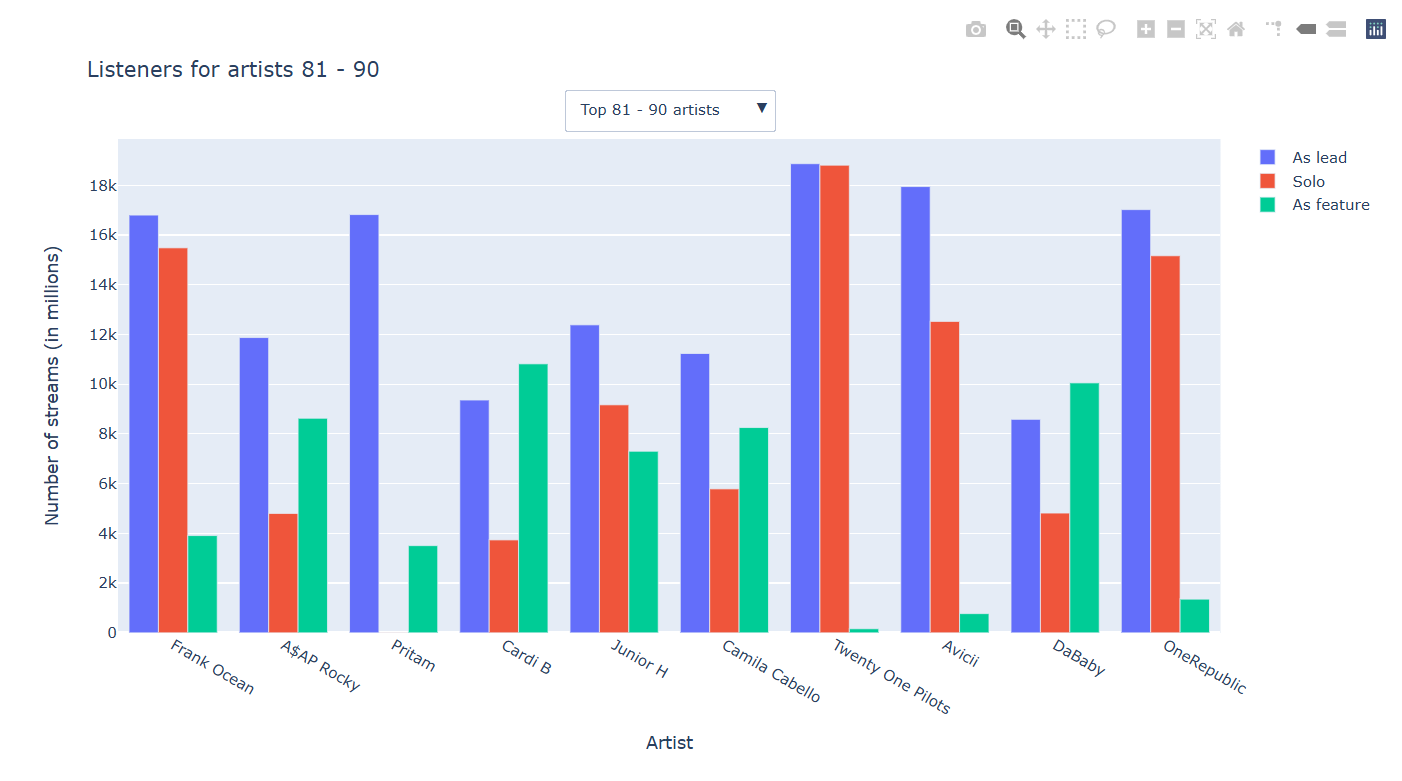
\includegraphics[width=\textwidth]{data/report_figures/graph7_spotify.png}
        \caption{Top 81-90 Artists}
        \label{fig:spotify7}
    \end{subfigure}
    \vskip\baselineskip
    \begin{subfigure}[b]{0.8\textwidth}
        \centering
        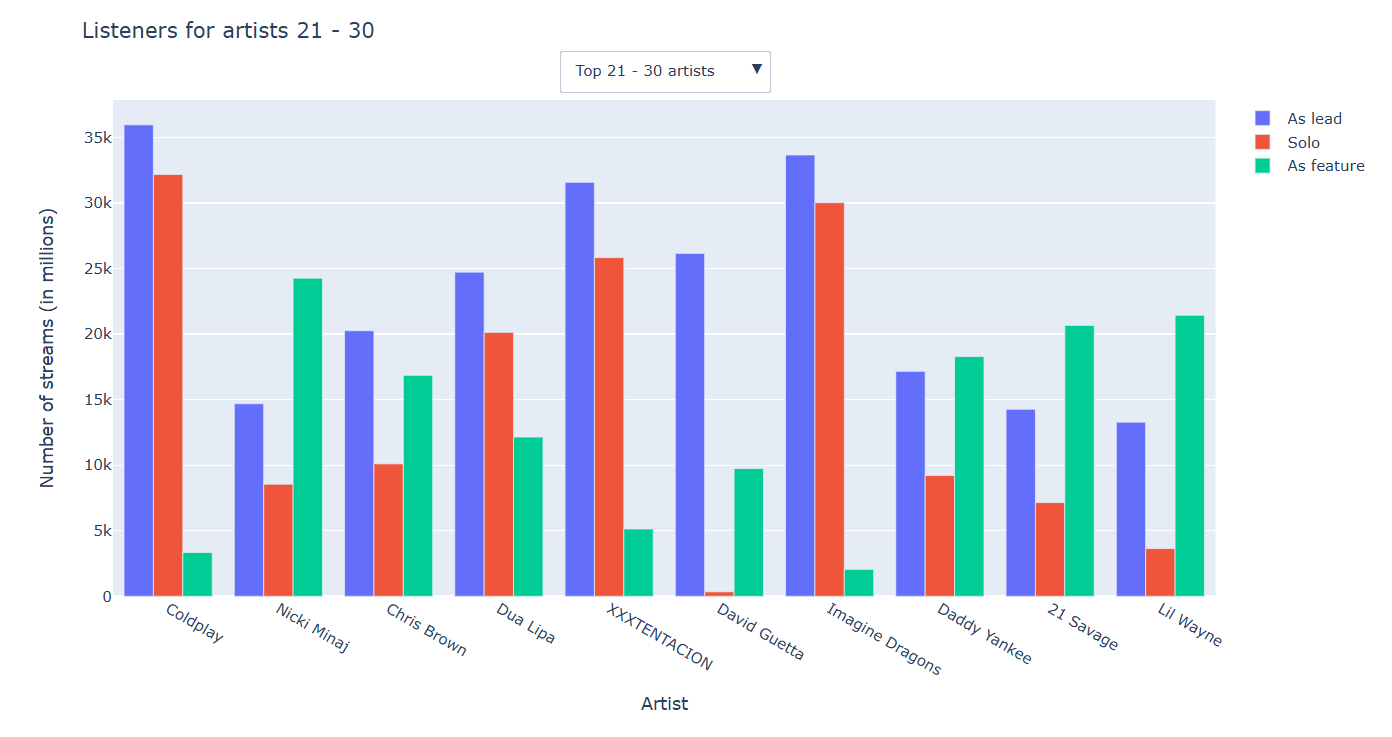
\includegraphics[width=\textwidth]{data/report_figures/graph8_spotify.png}
        \caption{Top 21-30 Artists}
        \label{fig:spotify8}
    \end{subfigure}

    \caption{\textbf{Number of collaborations depending on musical genre} \\ 
    The graphs show roughly similar trends. But we will look specifically at the top one. It can be seen that artists with a newer and more popular sound (hip-hop, pop songs) have many more collaborations than groups or musicians of older genres. This speaks of many things: the simplification of music in general (after all, it is much harder for rock groups to collaborate, and the genre itself is more protest and conflict-ridden), and a technological breakthrough, and globalization and the desire to "absorb" a large part of the music industry. For example, two groups stand out here: ASAP Rocky, Cardi B and DaBaby (many collaborations) and 21 Pilots and OneRepublic with almost zero joint songs.}
    \label{fig:spotify_combined3}
\end{figure}

\clearpage

\begin{figure}[htbp]
    \centering

    \begin{subfigure}[b]{0.8\textwidth}
        \centering
        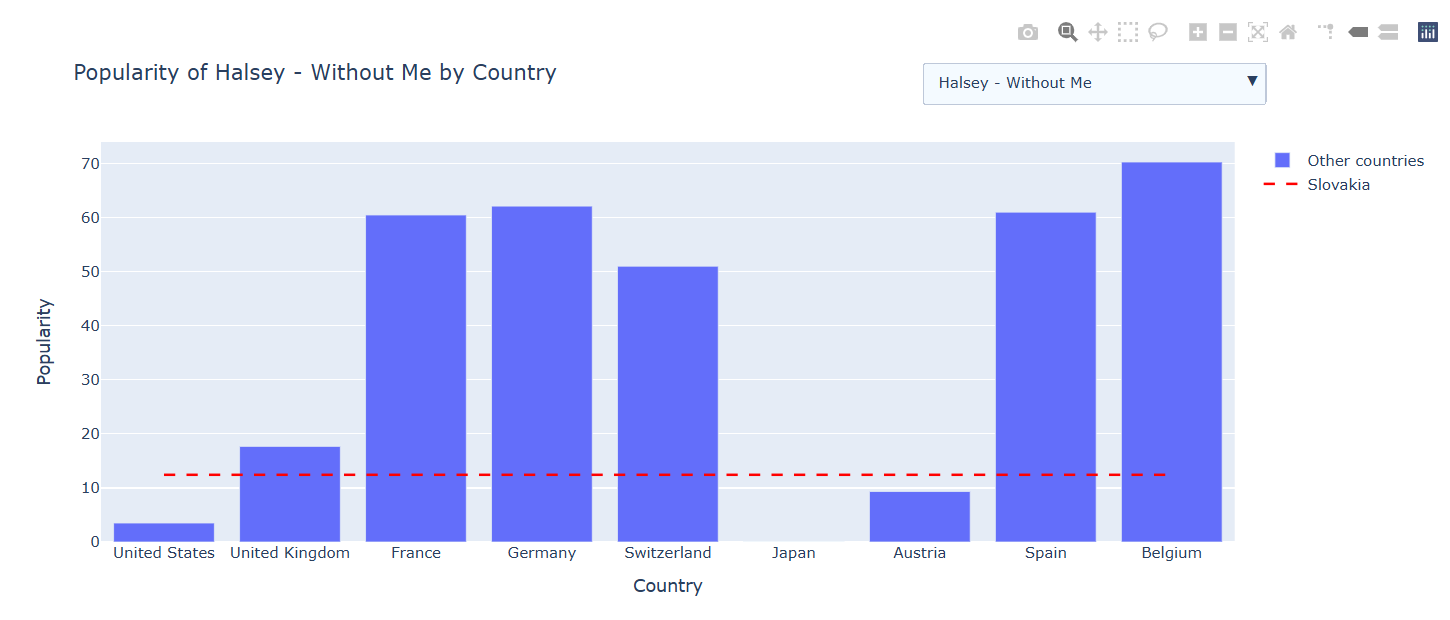
\includegraphics[width=\textwidth]{data/report_figures/graph2_itunes.png}
        \caption{Halsey - Without Me}
        \label{fig:itunes2}
    \end{subfigure}
    \vskip\baselineskip
    \begin{subfigure}[b]{0.8\textwidth}
        \centering
        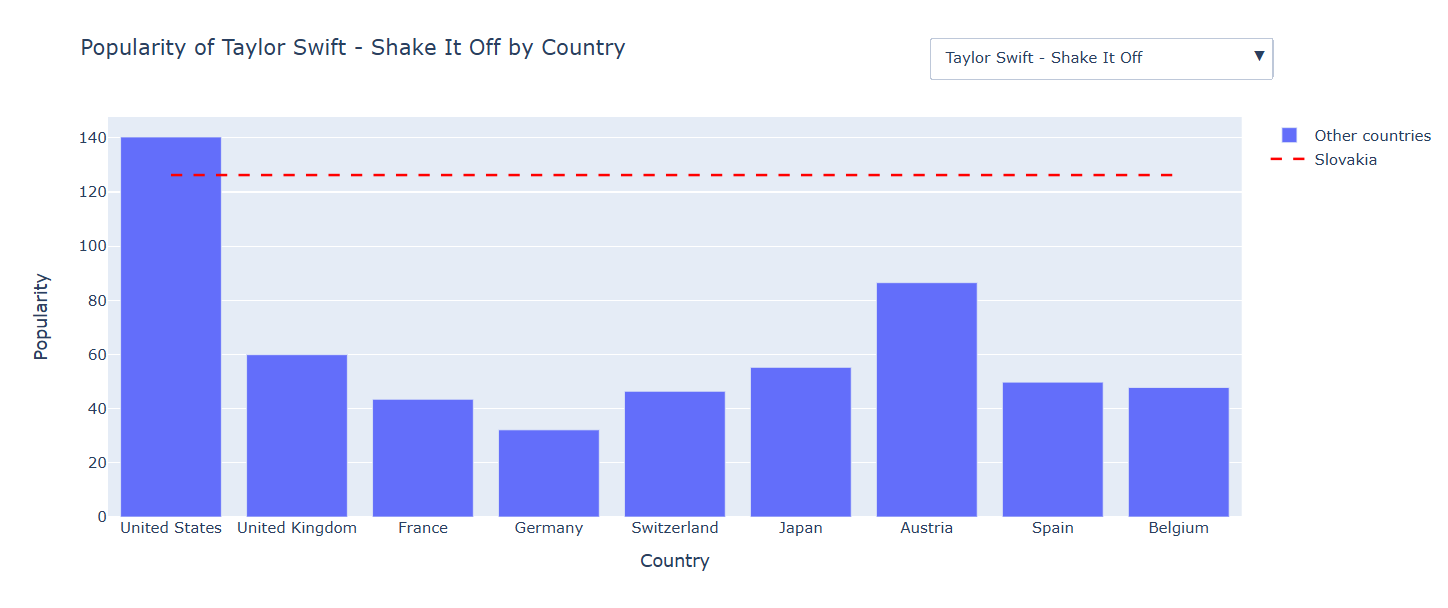
\includegraphics[width=\textwidth]{data/report_figures/graph3_itunes.png}
        \caption{Taylor Swift - Snake It Off}
        \label{fig:itunes3}
    \end{subfigure}

    \caption{\textbf{Track`s popularity by country} \\ 
    I am far from sure of these dependencies and correlations, but the following can be stated: cultural identity and nationality play a significant role in the formation of musical preferences. For example, in the graph above you can see the popularity of the song Halsey - Without Menya in different countries. The artist herself, performing the song, is bisexual. And the most interesting thing is that the song is very popular in Western European countries. Perhaps liberal views are reflected in musical preferences, but it is very difficult to say due to the lack of data + the listeners themselves may not know about the biography of the artist, and the track itself is quite popular. In the graph below you can see the distribution for the song Taylor Swift - Snake It Off. And here the American audience exceeds all the others by several times. Despite the fact that she is American, I did not find this for the other tracks.\\\\
Citation: American symbol. Swift's early girl-next-door image made her "America's Sweetheart". Journalists associate Swift's fame with Americanism. According to Knibbs, with her second studio album Fearless (2008), Swift had become a "countrified celebrity solidified into industrial-grade American fame" due to her craftsmanship.}
    \label{fig:itunes_combined}
\end{figure}

\clearpage

\begin{figure}[htbp]
    \centering

    \begin{subfigure}[b]{0.8\textwidth}
        \centering
        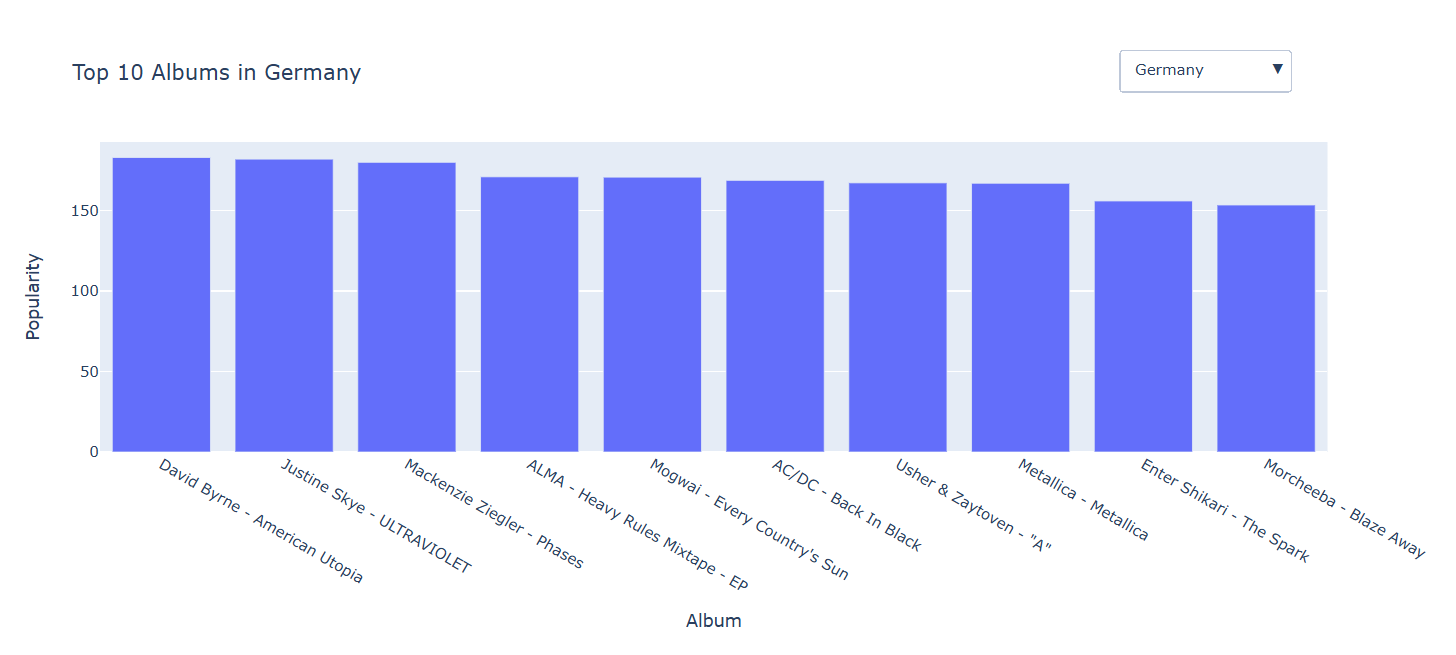
\includegraphics[width=\textwidth]{data/report_figures/graph1_apple_music.png}
        \caption{Germany - Top 10 Albums}
        \label{fig:apple_music_germany}
    \end{subfigure}
    \vskip\baselineskip
    \begin{subfigure}[b]{0.8\textwidth}
        \centering
        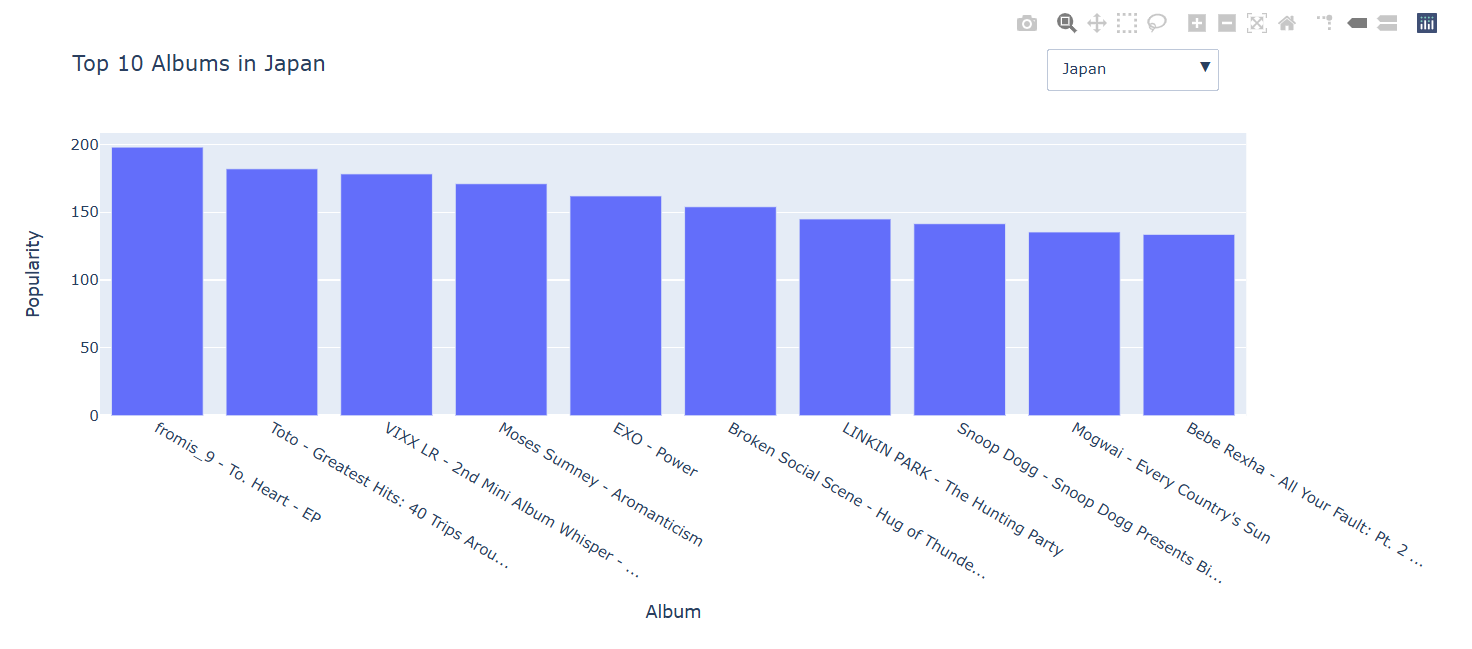
\includegraphics[width=\textwidth]{data/report_figures/graph2_apple_music.png}
        \caption{Japan - Top 10 Albums}
        \label{fig:apple_music_japan}
    \end{subfigure}

    \caption{\textbf{The Most Popular Albums in Different Countries} \\ 
    Continuing with the cultural specifics and differences, we can compare these graphs describing the top 10 albums by listening in Germany and Japan. We notice a significant number of rock albums in the German top, yet no Rammstein. This may be linked to globalization and market displacement, even for internationally known bands. In contrast, Japan’s chart features South Korean pop groups like fromis\_9 and VIXX LR, showing how cultural exports like K-pop penetrate other regions.}
    \label{fig:apple_music_combined}
\end{figure}

\clearpage

\begin{figure}[htbp]
    \centering

    \begin{subfigure}[b]{0.8\textwidth}
        \centering
        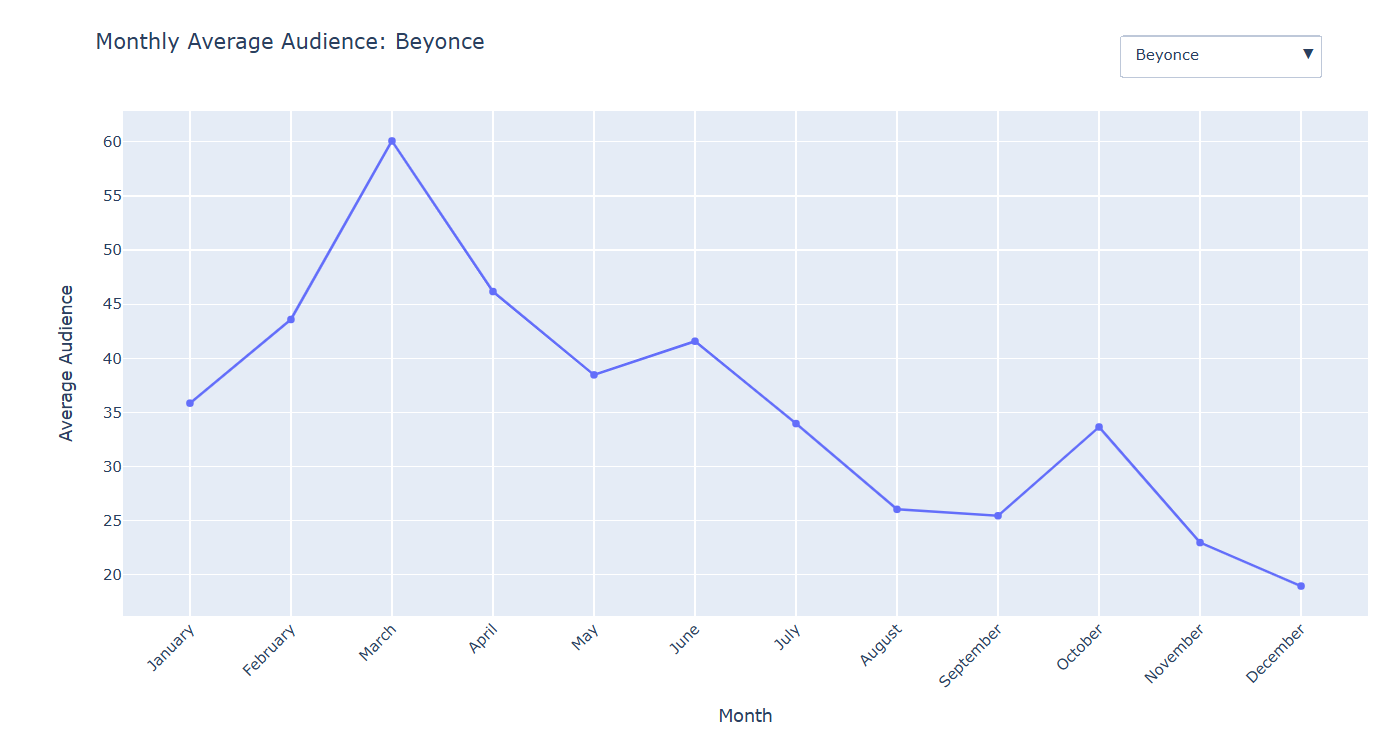
\includegraphics[width=\textwidth]{data/report_figures/graph1_radio_youtube.png}
        \caption{Beyonce}
        \label{fig:radio_youtube1}
    \end{subfigure}
    \vskip\baselineskip
    \begin{subfigure}[b]{0.8\textwidth}
        \centering
        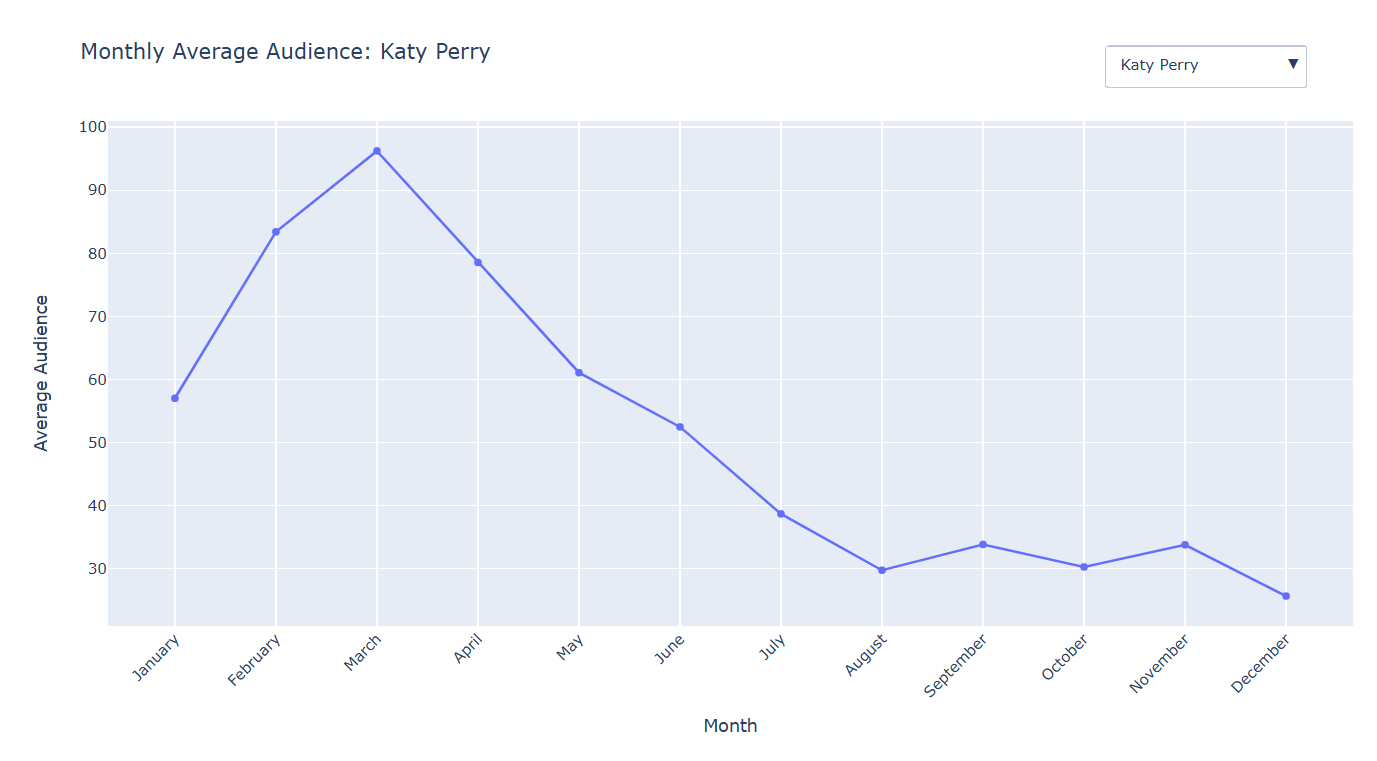
\includegraphics[width=\textwidth]{data/report_figures/graph2_radio_youtube.png}
        \caption{Katy Perry}
        \label{fig:radio_youtube2}
    \end{subfigure}

    \caption{\textbf{Pop Artists - Monthly Average Listeners} \\ 
    The next thing that interested me was the dependence of the popularity of an artist of a certain genre on the time of year or month. The data was taken specifically from a radio dataset, because it would be the most relevant in this case. In this graph, you can see how, approximately in the spring - by the beginning of summer, the number of listens of artists, mainly bright pop genres, increases significantly. Of course, this can be linked to the work of the radio stations themselves, which adapt to these cycles. But it seems to me that the heightened psychological state before the beginning of summer and natural conditions also play a role.}
    \label{fig:apple_music_combined}
\end{figure}

\clearpage

\begin{figure}[htbp]
    \centering

    \begin{subfigure}[b]{0.8\textwidth}
        \centering
        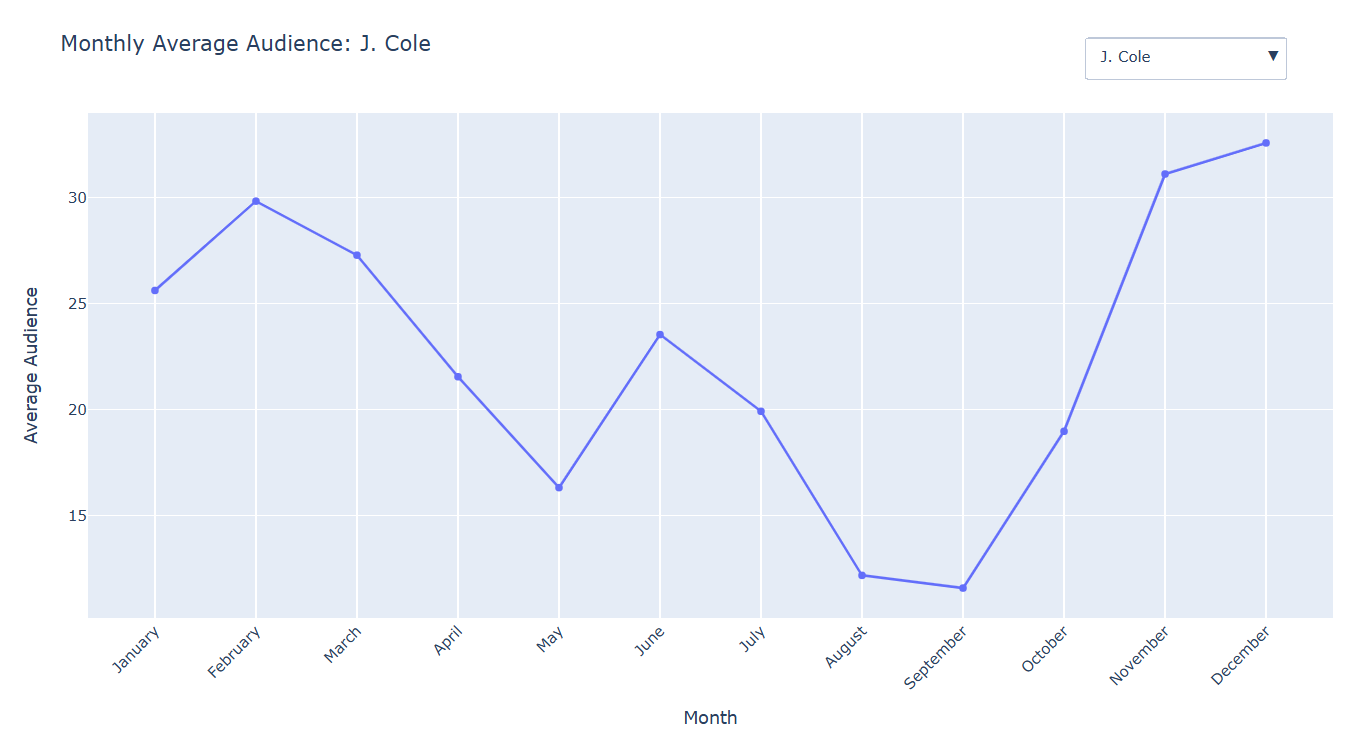
\includegraphics[width=\textwidth]{data/report_figures/graph5_radio_youtube.png}
        \caption{J. Cole (Hip-Hop)}
        \label{fig:radio_youtube3}
    \end{subfigure}
    \vskip\baselineskip
    \begin{subfigure}[b]{0.8\textwidth}
        \centering
        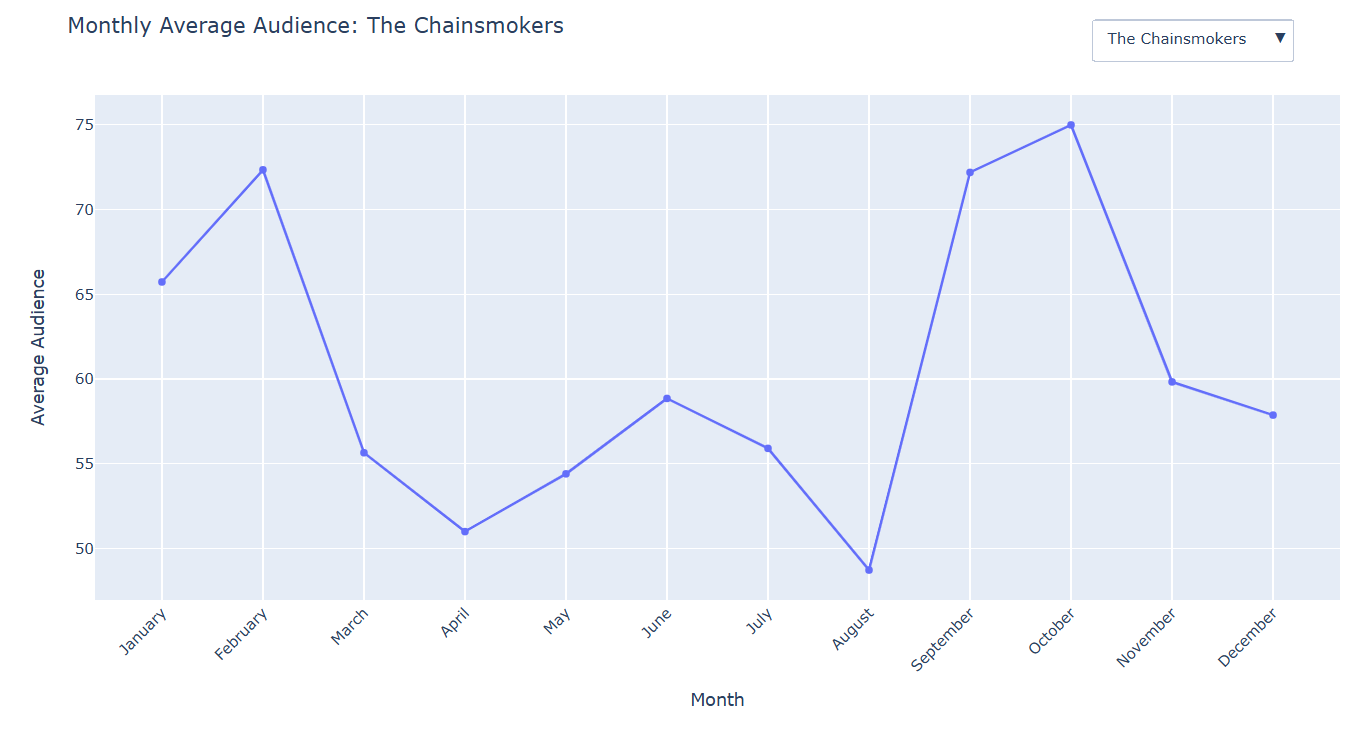
\includegraphics[width=\textwidth]{data/report_figures/graph7_radio_youtube.png}
        \caption{The Chainsmokers (Electronic)}
        \label{fig:radio_youtube4}
    \end{subfigure}

    \caption{\textbf{Rap/Electronic - Monthly Average Listeners} \\ 
    To make sure that the popularity of songs of certain genres depends on time conditions, I decided to take opposite genres: hip-hop and electronic music. Darker (and sometimes with lyrical lyrics (hip-hop)) musical genres begin to find a response closer to the end of autumn - the beginning of winter, which can really indicate a certain seasonality.}
    \label{fig:apple_music_combined}
\end{figure}

\clearpage

\begin{figure}[htbp]
    \centering

    \begin{subfigure}[b]{0.8\textwidth}
        \centering
        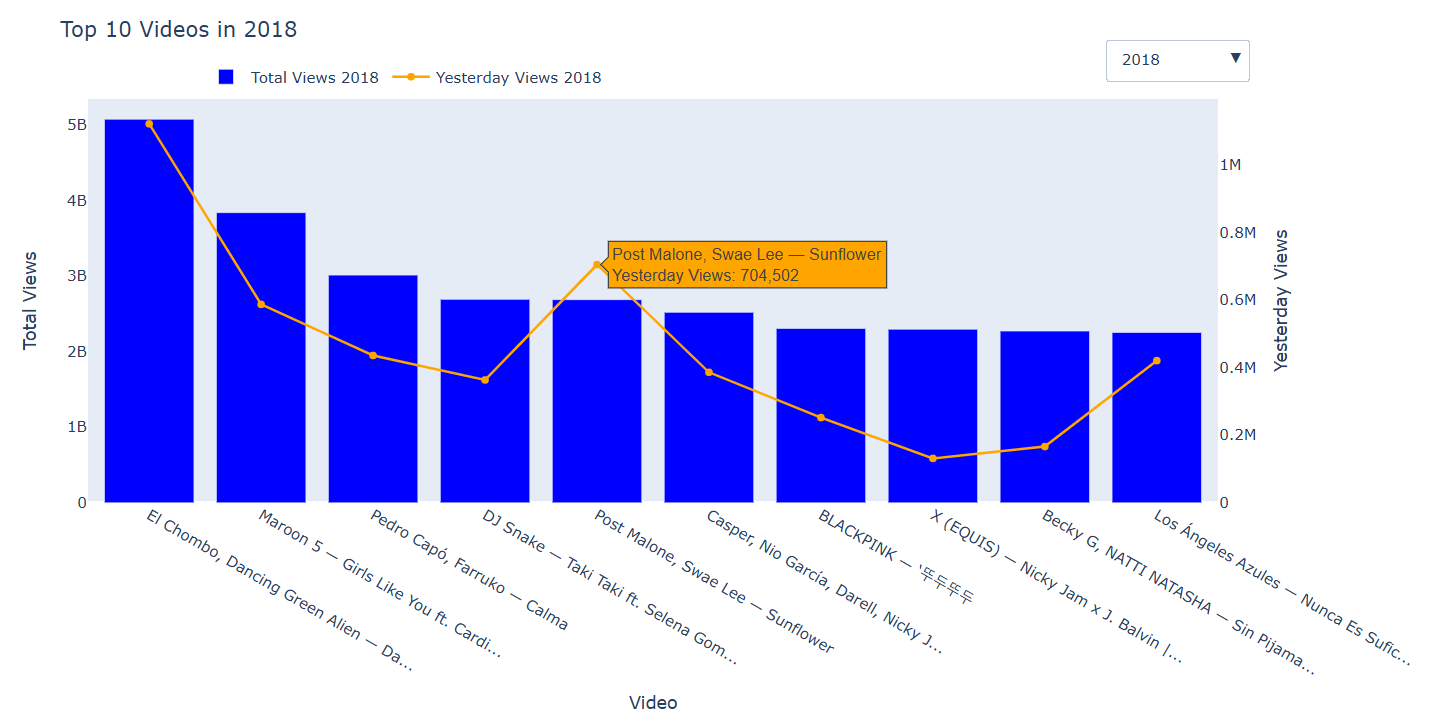
\includegraphics[width=\textwidth]{data/report_figures/graph9_radio_youtube.png}
        \caption{Top 10 Videos in 2018}
        \label{fig:video_2018}
    \end{subfigure}
    \vskip\baselineskip
    \begin{subfigure}[b]{0.8\textwidth}
        \centering
        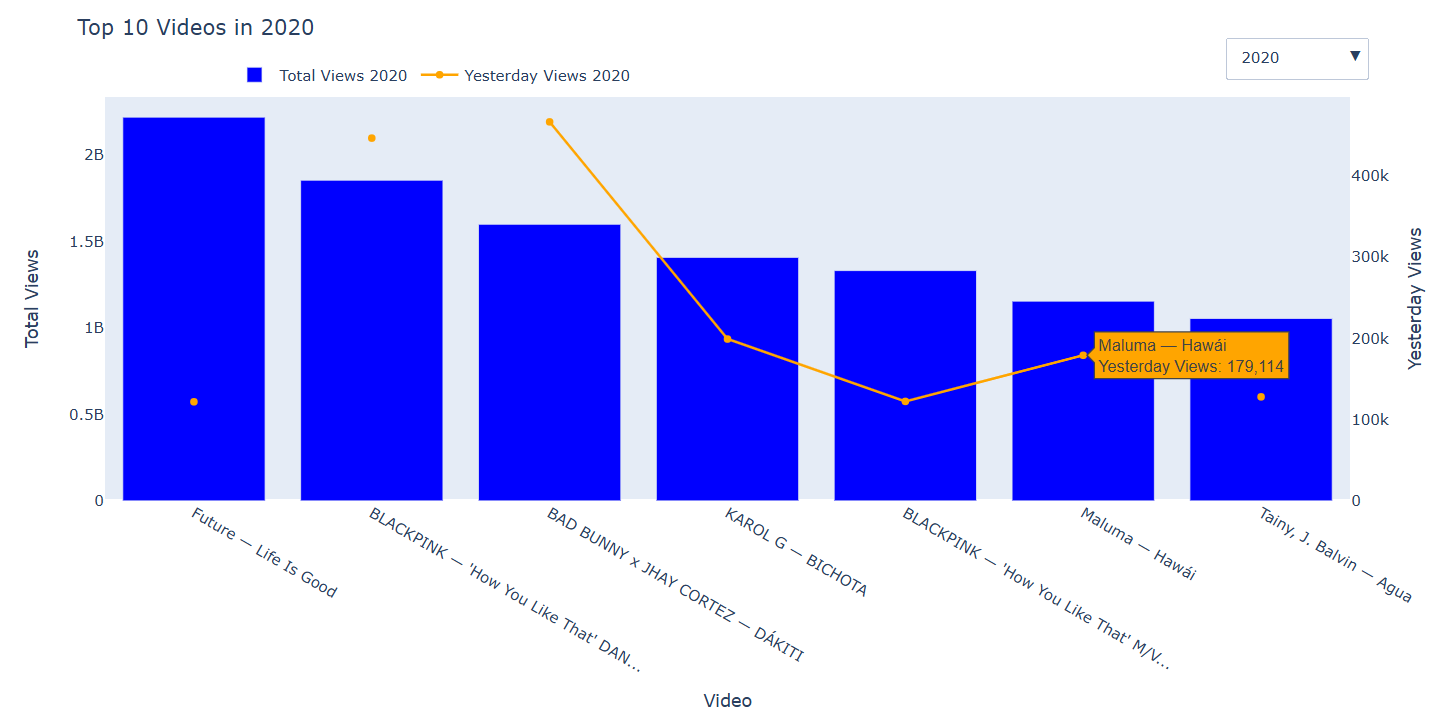
\includegraphics[width=\textwidth]{data/report_figures/graph8_radio_youtube.png}
        \caption{Top 10 Videos in 2020}
        \label{fig:video_2020}
    \end{subfigure}

    \caption{\textbf{Changes in Popularity of Music Videos Between 2018 and 2020} \\
The initial goal was to find correlations in the popularity of clips depending on the year. The hypothesis was that with the development and increasing availability of the Internet, older clips would be watched less than newer ones. In reality, there is no clear connection — if anything, the relationship is slightly inverse. This may suggest that people are growing tired of music videos, which are no longer as surprising or engaging as they once were. It might also relate to the rise in popularity of short-form video content. However, the graph tells a different story: in 2020, the number of views noticeably decreased, especially in the “Yesterday” column, which should reflect a video's current relevance. In previous years, these values were typically around 300–500 thousand views; in the pandemic year, they dropped to 100–200 thousand. One possible explanation is that the quality, budgets, and production teams behind music videos were significantly cut after the onset of COVID-19 and the resulting economic crisis.}
    \label{fig:video_popularity_2018_2020}
\end{figure}

\clearpage

\begin{figure}[htbp]
    \centering
    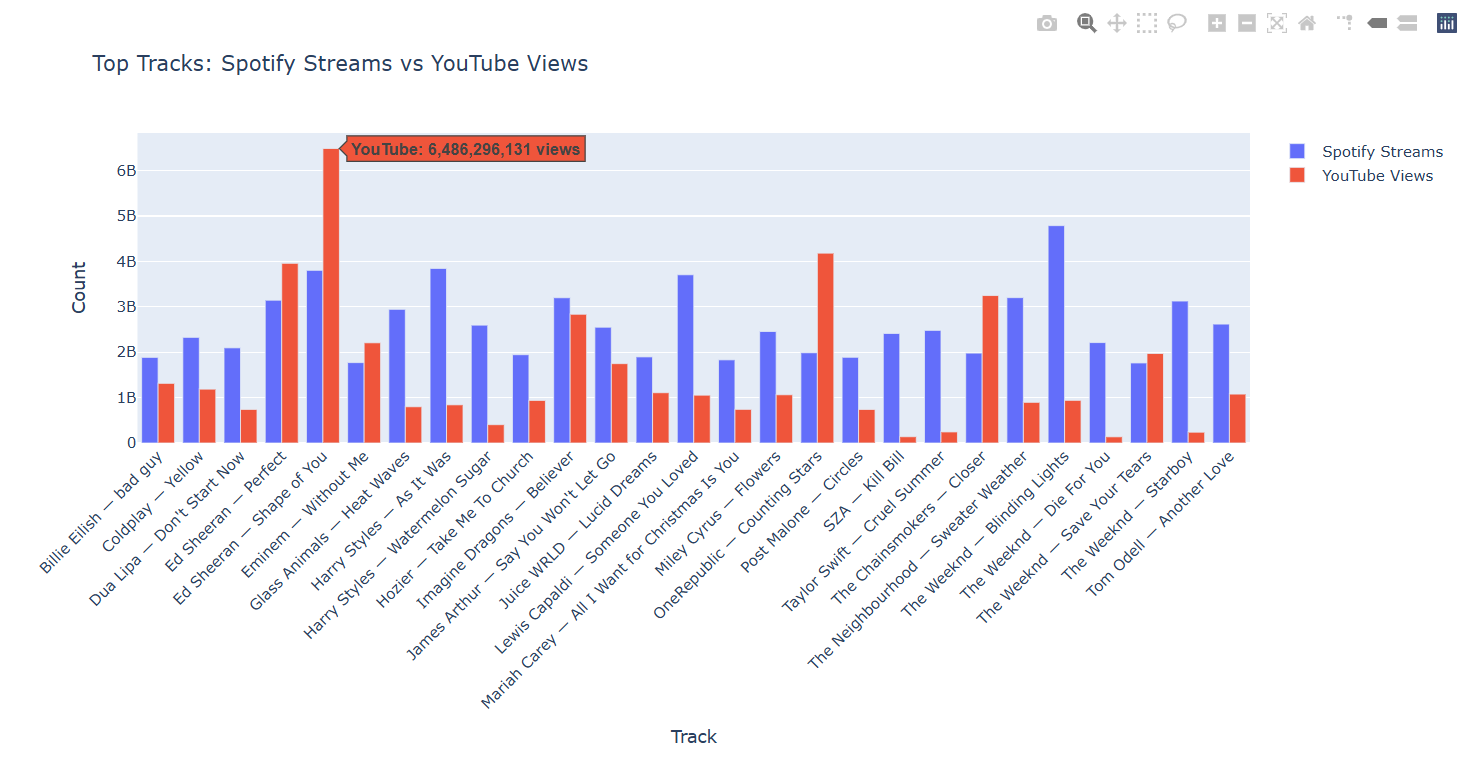
\includegraphics[width=0.8\textwidth]{data/report_figures/graph10_radio_youtube.png}
    \caption{\textbf{Spotify track streams and YouTube video clip views - Comparsion} \\
    This graph clearly shows that streaming services, despite appearing relatively recently, have already displaced YouTube as the primary platform for listening to music. Aside from 2–3 exceptions (such as Ed Sheeran's "Shape of You"), most tracks have significantly more streams on Spotify. This is expected — it’s much easier for people to use a dedicated music service to listen to songs without needing to play a video.\\
\textit{Upd.} I had to choose green as the color for bars representing Spotify streams.}
    \label{fig:youtube_final}
\end{figure}

\clearpage

\section*{Conclusion}

It seems to me that these graphs have shown quite well how people's musical preferences in a certain place and time can change or adapt to global trends, and that music is not a phenomenon that flows independently. Unfortunately, in my opinion, the market situation and conveyor-style production have long begun to suppress music and real art, which once required incredible effort. I really want to believe that this trend will decline in the near future, but with the Internet penetrating more households and lives, this seems unlikely.

As for the technical aspects during the implementation of this project, the most difficult part was coming up with interesting relations and trying to create meaningful graphs. Unfortunately, I slightly miscalculated the data selection — I chose a large dataset with only a small number of truly interesting attributes. Nevertheless, I tried to extract as much value from them as possible. Parsing the website was also unpleasant, but simultaneously the most interesting part. I got acquainted with the dynamic parser Selenium, which also opened the door to learning web testing in general. The easiest step was probably cleaning the data — it was relatively clean to begin with.

(I am writing this at 5:27 AM on June 16. (current project size: 1Gb)) To be honest, I really wish I had read the instructions before starting the project and chosen a much smaller dataset.


\end{document}